\section{Bezier}

Uma curva bezier pode ser definida por um qualquer numero de pontos, pontos estes chamados pontos de controlo da curva. Transformações como translação e rotação podem ser aplicadas na curva manipulando estes pontos. 

O algortimo de Casteljau oferece uma construção geométrica de onde se pode dividir uma curva de Bezier em duas curvas Bezier num parâmetro arbitrário t [0,1]. Como se pode observar:

\begin{center}
 	
 	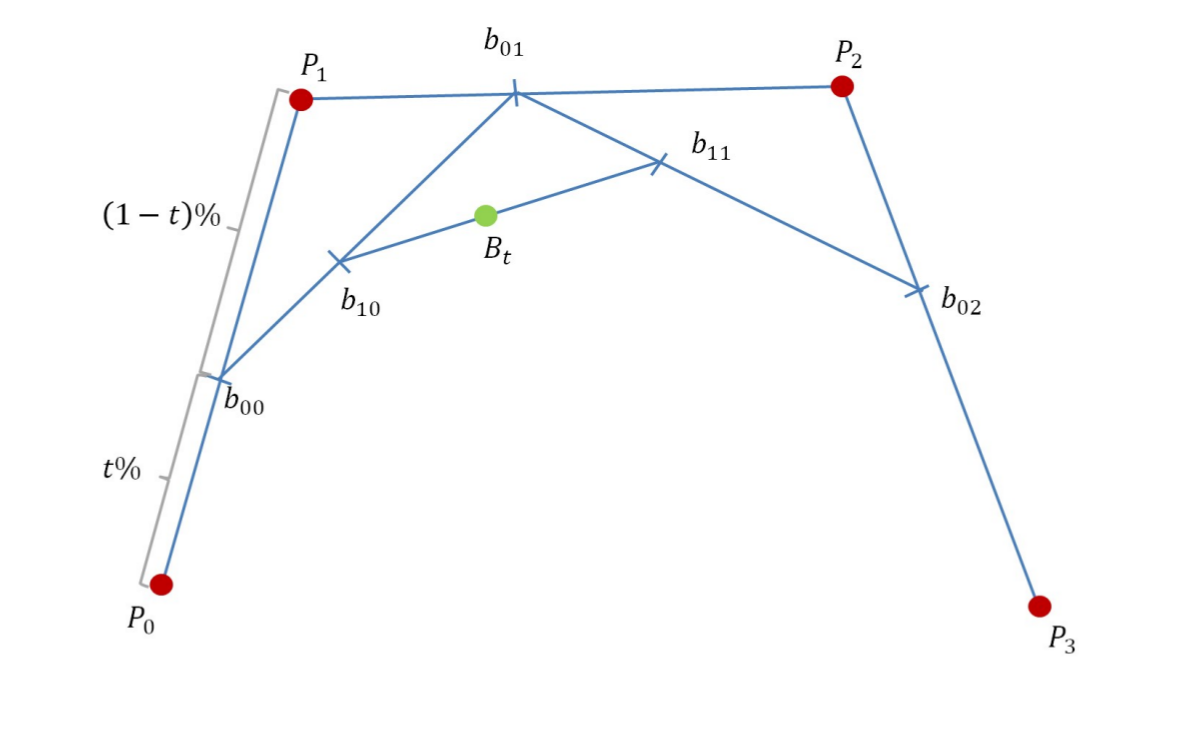
\includegraphics[scale=1.5,keepaspectratio]{resources/casteljou.png}
 	\captionsetup{type=figure, width=0.8\linewidth}
	\caption{Algoritmo geométrico casteljou.png}
\label{fig:ssec1:diagram:plane:to:sphere} 
\end{center}

Fazendo os cálculos manualmente 
\begin{center}
 	
 	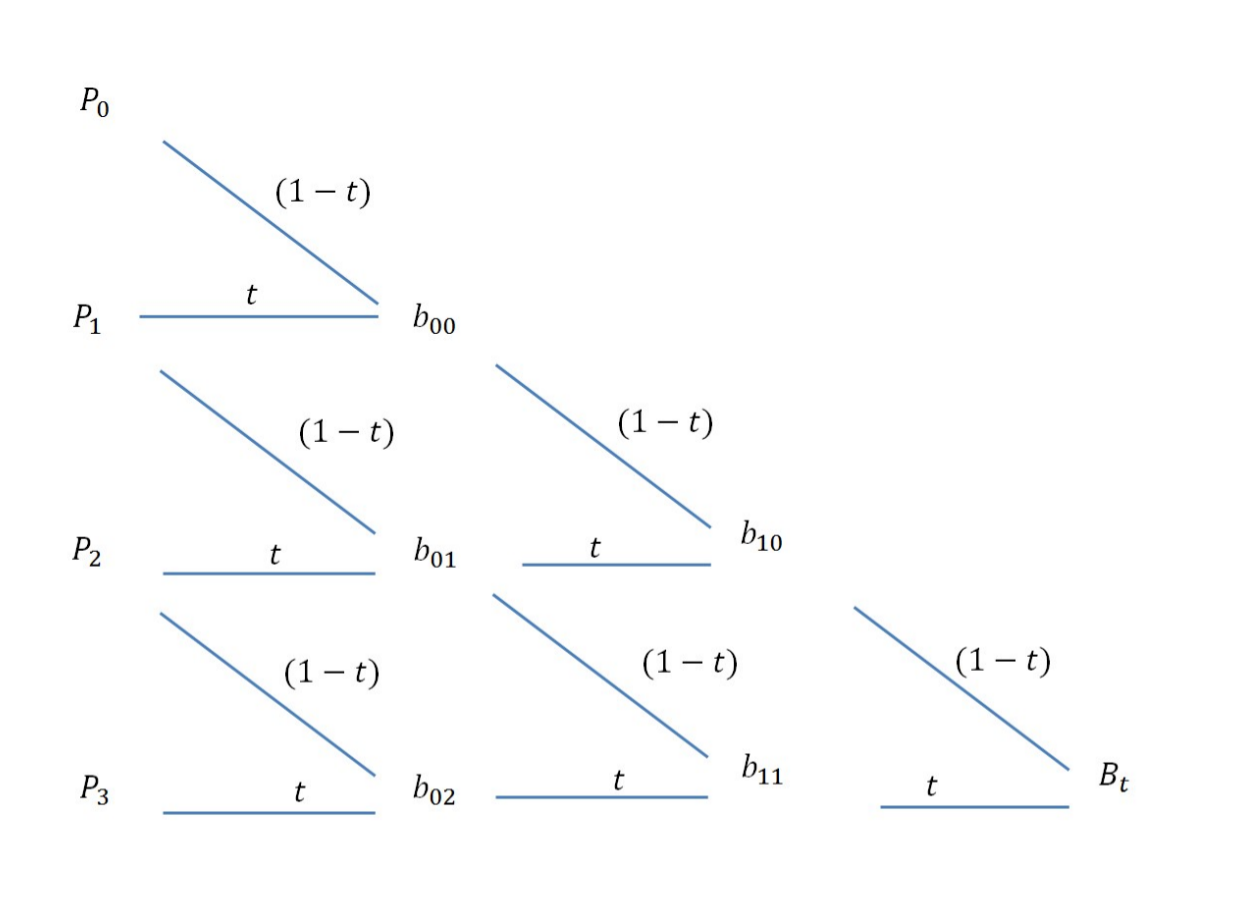
\includegraphics[scale=1.5,keepaspectratio]{resources/casteljeau2.png}
 	\captionsetup{type=figure, width=0.8\linewidth}
	\caption{Representação da árvore casteljeau}
\label{fig:ssec1:diagram:plane:to:sphere} 
\end{center}

Para demonstrar estras tranformações segue-se o exemplo de uma curva de bezier cúbica, isto é, uma curva definida por 4 pontos de controlo:

\begin{center}
 	
 	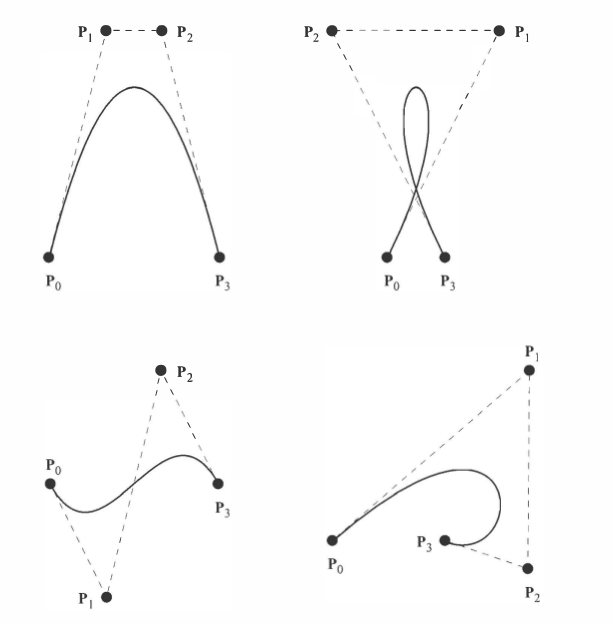
\includegraphics[width=\textwidth,height=\textheight,keepaspectratio]{resources/exemplos1Bezier.png}
 	\captionsetup{type=figure, width=0.8\linewidth}
	\caption{Curvas exemplo de Bezier}
\label{fig:ssec1:diagram:plane:to:sphere} 
\end{center}

Como se pode observar cada uma das curvas observadas possui 4 pontos de controlo, P0, P1, P2 e P3. A figura demonstra alguma das formas que uma curva de Bezier pode tomar. 
As curvas de Bezier, independentemente do número de pontos de controlo que possam ter, são sempre definidas pela seguinte fórmula:
\begin{equation}
B(t)=\sum_{k=0}^{n}B_{n,k}(t)P_{k}
\end{equation}

onde n corresponde a (nº pontos de controlo - 1), e t é o polinómio Bernstein que tem sempre um valor positivo em [0,1] e o seu somatório é sempre igual a 1.




Com 4 pontos de controlo, uma curva de Bezier diz-se cúbica e pode ser definida pela seguinte formula:




\begin{equation}
B(t)=\sum_{k=0}^{3}B_{3,k}(t)P_{k}
\end{equation}

\begin{equation}
B(t)=t^{3}P_{3}+3t^{2}(1-t)P_{2}+3(t(1-t)^{2})P_{1}+(1-t)^{3}P_{0}
\end{equation}




Quanto maior o número de pontos de controlo maior o custo computacional de as representar.